\section{Non $Z$+jets background processes}
\label{app:bkg-processes}

The event selection described in section~\ref{sec:selection} targets $Z\to\mu\mu$ in the high \pTll{} region. This results in an extremely pure sample of strong $Z\to\mu\mu$ production, which is the process used in the unfolding (see section~\ref{sec:mc}). To investigate the contribution from other processes, n-tuples from the VBF-Z analysis were used, which measured EW $Zjj$ production (``VBF-Z'') using both $\mu\mu$ and $ee$ data and MC. This analysis required two jets, however the n-tuples saved all events after the dilepton selection, so it was trivial to reported the event selection of this analysis. The only difference in event selection is that the VBF-Z analysis use dimuon trigger while this analysis use single muon triggers, which results in $~15$\% lower overall event yields. Table~\ref{tab:bkgProcesses} presents the observed and predicted event yields for a range of processes, and figure~\ref{fig:bkgProcesses} shows the \ptll{} and $m_{\mu\mu}$ distributions for each data taking period with the associated predictions.

\begin{table}[h]
  \centering
  \begin{tabular}{l|r|r|r|r|r|r|}\hline\hline
    Dataset   & \multicolumn{2}{c|}{2015+2016} & \multicolumn{2}{c|}{2017} & \multicolumn{2}{c|}{2018}\\ \hline
    $\ptll$ cut [GeV] & $> 165$ & $> 200$ & $> 165$ & $ > 200$ & $> 165$ & $> 200$ \\ \hline\hline
    Data                            &  89167 &  47544 &  103286 &  55132 & 138251 & 74197 \\ \hline
    Strong $Zjj$ (\sherpa{} 2.2.1)  &  79670 &  43295 &   95120 &  51520 & 125280 & 67430 \\ 
    Strong $Zjj$ (MG5 LO)           &  94430 &  51817 &  112450 &  61860 & 147310 & 81040 \\ \hline
    EW $Zjj$ (\powpy{})             &   1207 &    786 &    1431 &    928 &   1932 &  1260 \\ 
    $ZV$ $(V\to jj)$                &   1438 &    890 &    1718 &   1059 &   2261 &  1404 \\  
    Other $VV$                      &    511 &    308 &     606 &    367 &    811 &   497 \\ 
    $t\bar{t}$, single top          &    263 &     88 &     306 &    106 &    393 &   141 \\ 
    $W(\to\ell\nu)$, $Z(\to\tau\tau)$ &    3 &      2 &       0 &      0 &      3 &     3 \\ \hline
    Non-strong $Zjj$                &  3422  &   2074 &    4061 &   2460 &   5400 &  3305 \\ \hline
    Non-$Zjj$ / data                &  3.8\% &  4.4\% &   3.9\% &  4.5\% &  3.9\% & 4.4\% \\ \hline\hline
    \end{tabular}
    \caption{Observed and expected event yields following the event selection described in section~\ref{sec:selection} except using dimuon triggers instead of single muon triggers.}
    \label{tab:bkgProcesses}
\end{table}

\begin{figure}[p]
\centering
\includegraphics[width=0.48\textwidth,page=2]{figures/nonZjj_bkg_plots_VBFZ.pdf}
\includegraphics[width=0.48\textwidth,page=4]{figures/nonZjj_bkg_plots_VBFZ.pdf}
\includegraphics[width=0.48\textwidth,page=6]{figures/nonZjj_bkg_plots_VBFZ.pdf}
\includegraphics[width=0.48\textwidth,page=8]{figures/nonZjj_bkg_plots_VBFZ.pdf}
\includegraphics[width=0.48\textwidth,page=10]{figures/nonZjj_bkg_plots_VBFZ.pdf}
\includegraphics[width=0.48\textwidth,page=12]{figures/nonZjj_bkg_plots_VBFZ.pdf}
\caption{Predicted and observed \ptll{} and $m_{\mu\mu}$ spectra for each data taking period for data and a range of simulated processes.}
\label{fig:bkgProcesses}
\end{figure}



% 2016
% Data                 89167.00
% StrongSherpa         79673.02
% StrongMG             94432.74
% EW_Powheg            1206.67
% Top                  262.55
% Vjets                3.68
% DibosonZjj           1438.51
% DibosonOther         511.13

% 2017
% Data                 103286.00
% StrongSherpa         95120.53
% StrongMG             112448.75
% EW_Powheg            1431.02
% Top                  306.24
% Vjets                0.00
% DibosonZjj           1718.17
% DibosonOther         605.89

% 2018
% Data                 138251.00
% StrongSherpa         125281.99
% StrongMG             147311.15
% EW_Powheg            1931.96
% Top                  392.79
% Vjets                2.88
% DibosonZjj           2261.02
% DibosonOther         811.45